% Fitting-error definition in the form of Long 2016 dissertation Fig. 2.6(c).
% Standalone, Overleaf-ready (pdfLaTeX): only amsmath + tikz.
%   Delta B = B_fit - B_FEM   (per-point error vector)
%   Error % = |Delta B| / |B_FEM| * 100

\documentclass{article}
\usepackage{amsmath}
\usepackage{tikz}
\usetikzlibrary{arrows.meta}

\begin{document}

\begin{figure}[htbp]
\centering
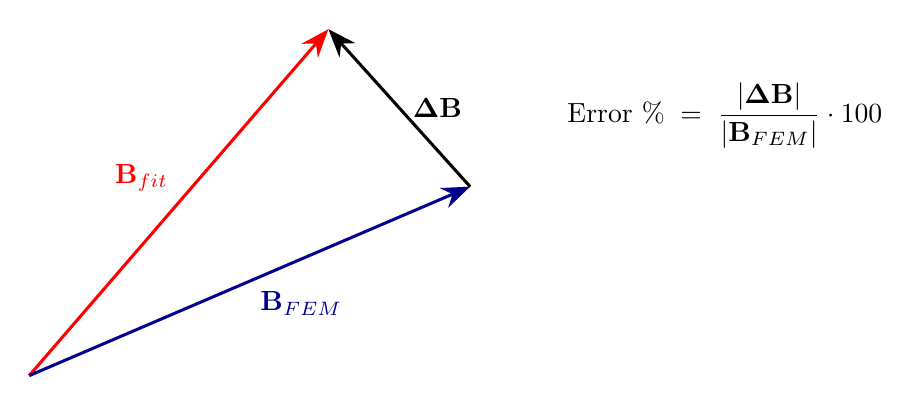
\begin{tikzpicture}[>={Stealth[length=3.6mm]}, line width=1.1pt]
  % common origin
  \coordinate (O) at (0,0);
  \coordinate (F) at (3.8,4.4);    % tip of B_fit
  \coordinate (M) at (5.6,2.4);    % tip of B_FEM

  % B_fit (red): origin -> F
  \draw[->, red] (O) -- (F)
        node[midway, above left] {$\mathbf{B}_{fit}$};

  % B_FEM (dark blue): origin -> M
  \draw[->, blue!55!black] (O) -- (M)
        node[midway, below right] {$\mathbf{B}_{FEM}$};

  % Delta B (black): tip of B_FEM -> tip of B_fit  (= B_fit - B_FEM)
  \draw[->, black] (M) -- (F)
        node[midway, right=1pt] {$\boldsymbol{\Delta}\mathbf{B}$};

  % error formula
  \node[anchor=west] at (6.7,3.3)
     {$\displaystyle \text{Error \%} \;=\; \frac{\lvert\boldsymbol{\Delta}\mathbf{B}\rvert}{\lvert\mathbf{B}_{FEM}\rvert}\cdot 100$};
\end{tikzpicture}

\caption{Definition of the fitting error (after Long 2016, Fig.~2.6(c)).
The error vector is $\boldsymbol{\Delta}\mathbf{B} = \mathbf{B}_{fit} - \mathbf{B}_{FEM}$,
and the percent fitting error is
$\text{Error \%} = \lvert\boldsymbol{\Delta}\mathbf{B}\rvert / \lvert\mathbf{B}_{FEM}\rvert \cdot 100$.}
\label{fig:fitting_error_def}
\end{figure}

\end{document}
